\documentclass[conference]{IEEEtran}
\IEEEoverridecommandlockouts
% The preceding line is only needed to identify funding in the first footnote. If that is unneeded, please comment it out.
% \usepackage{cite}
\usepackage{xcolor}
\usepackage{listings}
\usepackage{amsmath,amssymb,amsfonts}
\usepackage{comment}
\usepackage{algorithmic}
\usepackage{tabularx}
\usepackage{multirow}
\usepackage{graphicx}
\graphicspath{ {./images/} }
\usepackage{textcomp}
\usepackage{xcolor}
\def\BibTeX{{\rm B\kern-.05em{\sc i\kern-.025em b}\kern-.08em
    T\kern-.1667em\lower.7ex\hbox{E}\kern-.125emX}}
\usepackage[
backend=biber,
style=ieee,
sorting=ynt
]{biblatex}
\addbibresource{export.bib}
\begin{document}

\title{MSc Research Report\\}

\author{
\IEEEauthorblockN{Seán Ó Fithcheallaigh (B00830189)}
\IEEEauthorblockA{\textit{Department of Computing} \\
\textit{Ulster University}\\
Belfast, N. Ireland \\
o\_fithcheallaigh-s@ulster.ac.uk}
}

\maketitle

\begin{abstract}
TBD
\end{abstract}

\begin{IEEEkeywords}
Machine Learning, Deep Learning, Embedded Systems, The Edge, Neural Networks, Arduino
\end{IEEEkeywords}

\section{Introduction}
This project is related to the testing and development of an obstacle avoidance and navigation system for people with sight difficulties. The initial part of this section will give background information on why systems like this are needed, and will then move into a more detailed exploration of the project.
\subsection{The lives of people dealing with sight loss}
There are over two million people in the UK who are living with sight loss; where sight loss includes: people who are registered blind or partially sighted; people whose vision is better than the levels that qualify for registration; people who are awaiting or having treatment such as injections, laser treatment or surgery that may improve their sight; Correctly prescribed glasses or contact lenses could improve the sight of people who have sight loss \cite{rnib}. Experts also predict that the number of people suffering from sight loss will double to over four million by 2050 \cite{Pezzullo}.

Of the two million people with sight loss, the leading causes of sight loss include (with the approximate number of people affected) \cite{rnib}:
\begin{itemize}
    \item Age-related macular degeneration (AMD) (488,000 people)
    \item Cataract (394,000 people)
    \item Diabetic retinopathy (97,000 people)
    \item Glaucoma (151,000 people)
    \item Uncorrected refractive error (809,000 people)
    \item Other eye problems (150,000 people)
\end{itemize}


How sight loss impacts those effects can vary, depending on personal circumstances. Some factors which can be influential in a person's experience with sight loss can be: they receive support and receive it at the right time, a person's age, the presence of other disabilities, and the severity of the sight loss. However, most people in the UK agree that those with visual impairments are not treated the same as those without visual impairments, according to a key finding in [1].

People with visual impairments are less likely to go into an environment with which they are not familiar. As a result, visual impairments can have a negative impact on their health and well-being. Obstacle detection and warning can improve the mobility and safety of visually impaired people, particularly in unfamiliar environments; as one RNIB research participant said, "If there were more things in shops to help people with sight loss [...] to help us get around" [1]. However, if we look around our world, we can see that transport systems are not built with the visually impaired in mind [3]. This fact is one factor likely to be a factor in four out of every ten blind people who are only able to make some of the journeys they either need to or wanted to \cite{rnib}.

Visually impaired people face many issues when navigating their journey, such as understanding how to reach their destination. Typically, the route to a destination will stay the same - streets remain in the same place, and road crossings tend not to move. However, another issue they face is random obstacles placed in their path. These are things that a visually impaired person could have no way to know is there. Of course, items such as the white cane some blind people use can assist with this kind of issue. However, not everyone may want to use a cane (potentially because of the signal that sends: I am different, I have an impairment), and potentially because, if registered as blind, many people still have some level of vision and do not wish to give up a level of independence completely. 

\subsection{The Problem}
A need exists to develop systems that can assist visually impaired people in navigating their surroundings. In any proposed navigation system for the visually impaired, obstacles must first be detected and localised. Then, navigation information must be communicated to the person, allowing them to avoid obstacles. Using various modalities such as voice, tactile feedback, and vibration could facilitate the achievement of this goal.
 
This project proposes using machine learning (ML) methods within an embedded system to develop a solution that can detect obstacles in the path of a visually impaired user navigating an indoor environment. 
 
Several tasks will need to be completed to determine the system's feasibility. The first step will be the investigation of various sensor modalities in order to determine the most appropriate sensor or combination of sensors. Then a dataset will be gathered covering a range of obstacle detection and avoidance scenarios. This dataset will then be used to train, test, and validate several Deep Learning (DL) and ML models to understand which is best at detecting and localising obstacles. Development work will then be done to allow this model to be implemented on a constrained device, and the performance of the final model will be assessed against critical parameters.
This paper will detail this work by covering the main steps listed above. 

\section{Technical Review}
\subsection{Introduction}
This section of the report will present a background discussion on the technical aspects of this project. 

As has been discussed, the goal is to design and build an object detection system which researchers can implement on a constrained device. This detection system will operate at what is called "the edge". This section of the report will start with a discussion of what is meant by the edge, covering the advantages and disadvantages of working at the edge and the hardware and software considerations required. 

\subsection{The Edge}
In recent years, the term "edge" has been coming up more and more in discussions about the future directions of machine learning ML, and is often discussed in connection with the Internet of Things (IoT). When discussing machine learning at the edge, one may hear terms such as "edge AI" or "edge ML". Other standard terms would be "embedded machine learning", "embedded ML", "embedded AI", and a popular phrase: "tiny ML". All these terms are interchangeable, and while there may be some differences depending on the context, a person can use any of these terms to discuss the same topic.

Embedded is quite a common term in the field of electronic engineering. An embedded device, or an embedded system, is a computer that controls the electronics of many of today's modern devices. We can find embedded systems in everything from mobile phones to modern cars to satellites which orbit the Earth. These embedded systems can run software that will control the system's functions and ability.
Embedded systems are in more places than one may imagine, or it may be more accurate to say that there are more embedded chips in a single device than one may imagine. Globally, In 2020, more than 28 billion microcontrollers were shipped, and the trend is predicted to grow, with a focus on automation and AI devices \cite{ucmarket}. Given how common these devices are, it is pretty apparent that researching how best to transfer ML models to these systems is an important step.

The term 'edge' may seem slightly unusual. So how does edge relate to ML? 

When discussing the internet, computers, or IT systems, most people will have an image of their PC at home or the computer they use at work. However, there are more devices connected to the internet than computers. As of 2021, research shows there were 12.2 billion active IoT connections \cite{ucmarket}. These IoT devices cover almost any aspect of our lives that one cares to think about, everything from smartwatches; intelligent kitchen appliances; baby monitors connected to the internet, allowing parents to check in from anywhere in the world; shipping containers; and industrial sensors used to monitor the health of machinery. The list goes on and on.

How are all these billions of devices connecting to networks and communication? They have connected to servers, and these are the servers which are often referred to as the "cloud".
These devices are connected to a network; they take readings from their sensors and send that information to a location where it can be stored and processed. From this perspective, these devices sit at the 'edge' of the network, hence the name.

\subsubsection{Edge AI}
For a long time, IoT devices have been seen as ways to collect data via onboard sensors. They would collect the data and transmit it back to a hub for processing. However, this approach is costly in several ways. First, it can cost a lot of money to transmit large amounts of data, due mainly to the connectivity and storage costs; there is also the issue that transmitting data is a highly power-hungry task for any battery-powered IoT device. Second, it is expensive in human time, too, because people will need to evaluate the data and process it, potentially making some decisions based on that data analysis.

Sending information back to a central location to be processed and then returning the result can take time, referred to as latency. The time required for this may only be a matter of seconds, which is acceptable for some applications, but would be too long for other applications where near-instant feedback is needed. An example of a time-critical system could be a system on an autonomous vehicle needing to react to traffic lights. The vehicle cannot wait a few seconds to determine if it is approaching a red light and needs to stop. 

\subsubsection{Hardware Consideration}
Edge AI is built on constrained devices, such as microcontrollers (MCU). Constrained devices, such as microcontrollers, are the primary platform for edge AI applications. The limited processing power, available memory and power consumption are the main factors constraining these devices. 

The image in Fig. \ref{fig:ucblock} shows a block diagram for an edge AI device:    
\begin{figure}[h]
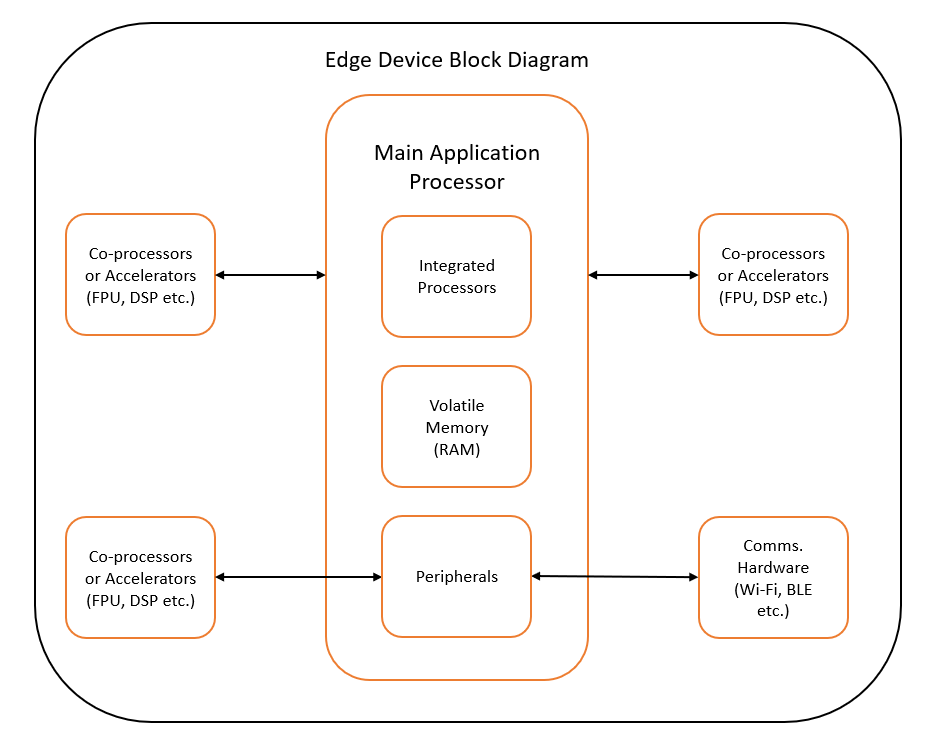
\includegraphics[width=8cm, height=6cm]{images/edge_device_block_diagram.png}
\centering
\caption{Block Diagram for a Constrained Device}
\label{fig:ucblock}
\end{figure}

Fig \ref{fig:ucblock} shows that the processor is the centre of the whole system, with the processor being the element that runs applications and runs the algorithm for an AI application. Depending on the system, there may also be co-processors or accelerators. An accelerator is a bit of hardware designed to carry out a specific task. For example, one typical accelerator would be a floating-point unit (FPU), which will be added to a system to carry out floating-point arithmetic as quickly as possible. Other accelerators which could be common in edge AI applications would be digital signal processing (DSP) blocks and linear algebra blocks \cite{edgeAI}. 

There are many edge AI devices that have been designed with a specific use case, or area of use, in mind. For example, there is the Carol \cite{carol}, which is a platform developed by Google for AI applications in a production environment. The System on Module (SoM) device is a fully integrated system for accelerated ML applications (including CPU, GPU, Edge TPU, Wi-Fi, and Bluetooth). The Jetson Nano from NVIDIA \cite{jetson}, which is an AI computer for makers, learners, and developers \cite{jetson1}. As discussed in \cite{jetson1}, the Jetson Nano allows for the use of libraries and APIs for TensorRT and cuDNN, which can be used for deep learning applications that require higher performance, CUDA for GPU accelerated applications, NVIDIA Container Runtime for containerised GPU accelerated applications, as well as APIs for sensor development or working with OpenCV. This, along with NVIDEA's other AI-focused development kits, is aimed at prototyping, before being put into production.

The systems mentioned so far would fall into the mid-to-high-end systems. However, lower-end systems are still capable of carrying out AI applications. One example of a lower-end system is the Beaglebone AI \cite{beagle}. This system is built on Linux, and based around the Texas Instruments (TI) AM5729, with a TI C66x floating point DSP, with TI embedded vision engines (EVE) \cite{tuomo}. Then there is the Arduino Nano 33 BLE Sense which is a small development board which is AI-enabled. The Arduino Nano 33 contains a number of onboard sensors, such as a 9-axis inertial sensor, humidity sensor, microphone and proximity sensor. The Arduino board also has GPIO pins which can allow extra sensors to be added if needed or required. The Arduino development kit allows for EML applications to be run where models created using TensorFlow Lite can be uploaded to the board via the Arduino IDE \cite{arduino}.

Another type of hardware configuration would be the field programmable gate array (FPGA). An FPGA is an IC which allows the user to configure the hardware to meet the requirements of the project. Using FPGAs allows the developer to build a processor that is specific and tailored to running ML models and so on. The flexibility that FPGAs allow means they are an excellent platform for developing AI accelerators \cite{tuomo}. Intel has a range of FPGAs which allow real-time, low-latency, and low-power deep learning inference. A number of devices such as the Intel Cyclone. Other manufacturers are producing AI-focused FPGAs, such as Qualcomm, which has, among other systems, the Snapdragon, which is a System on Chip (SoC) which contains a CPU and GPU and is very power efficient \cite{qualcomm}. 

\subsubsection{Software and Frameworks}
As previously discussed, when building edge AI applications on an MCU, one must give the availability of memory due consideration. Unfortunately, available memory is problematic when implementing any machine learning algorithm or neural network on an MCU because the weights and biases required for a model to function and any data points can take up large amounts of memory. Software libraries and frameworks have been developed to help reduce things like memory requirements.

The main tools or frameworks used in deep learning would be TensorFlow and its associated Keras API and PyTorch. Others like Theano, Caffe, and Microsoft CNTK are also available. TensorFlow, developed by Google Brian, is a powerful open-source library aimed at deep neural networks. These tools are typically optimised to run on GPUs and other specialised hardware. The reason for this is to accelerate the training processes. Once a model is trained, using that model to make inferences is less computationally expensive, which is essential for dealing with edge devices. However, it is important to note that why the inference is less computationally expensive, the MCU does not have a free ride - a reasonable amount of memory and processing power is still required to carry out the inference. To try and reduce the requirements on the front end, frameworks such as TensorFlow and PyTorch have implemented model compression techniques with little to no effect on computational accuracy \cite{tuomo}. 

While TensorFlow (with TensorFlow Lite) and PyTorch have been mentioned here, TensorFlow has been the main focus, because while PyTorch has PyTorch Mobile, it is aimed at mobile devices which run on either Android or iOS, whereas TensorFlow Lite can be used on embedded system \cite{tuomo} \cite{tfl1}.

\subsection{Tensor Flow Lite}
TensorFlow Lite (TLF) is a set of tools that have been designed and built to allow on-board machine learning. It has been designed to help developers run models on embedded systems, as well as on mobile devices [10].

Some of the key features of TensorFlow Lite (TFL) include:

\begin{itemize}
    \item Optimisation
    \item Multi-platform
    \item Multi-language options
    \item High performance
\end{itemize}

Process optimisation is extreme;y important when developing embedded machine learning (EML) systems. TFL deals with optimisation by dealing with a number of key constraints which are common to embedded systems: latency, privacy, connectivity, size, and power consumption \cite{jetson1}. The reduced latency comes from the fact that there is no information going to the server to be processed, and then back to the device. TFL removes a lot of privacy issues which may traditionally have been present in cloud-based ML tasks because no data will actually leave the device. Connectivity issues are side-stepped because the device does not need to connect to a network. Some systems may send information back to a cloud-based server, but this would become a non-critical task, in terms of timing. TFL can also reduce the size of any associated files, meaning they are more suitable for embedded applications. Power consumption is reduced through efficiencies in the interface, as well as the lack of network connection, since, typically, sending information tends to be a large drain on power.

On the topic of multi-platform, TFL can be used to develop models that will work on Android and iOS devices, as well as on MCU and embedded Linux systems. In terms of languages, TFL has support for Python, Objective-C, C++, Java and Swift. The ability to use multiple languages is a great advantage, but the ability to optimize the models is essential to the success of TFL. This will be discussed in the following section.

\subsubsection{Optimisation} Since optimisation is key, this section will explore the topic more. Various optimisation techniques can be applied to models to allow efficient operation with the limited computational power and limited memory available on a constrained device. As previously discussed, some optimisation techniques allow for the use of accelerated inference \cite{tfl2}.

Models should be optimised for a number of reasons. One of the main reasons would be size reduction. There is no single method used for reducing the model size, but no matter the process, there are a number of advantages in doing this:

\begin{itemize}
    \item \textbf{Smaller storage size}: A smaller size model will take up less memory on the end device. If we take the Arduino Nano as our target device, this MCU does not come with a lot of onboard memory, so reducing the model size is critical for deployment.
    \item \textbf{Reduced memory usage}: Using a smaller model will result in less RAM being used when the model is run. This will allow other more memory to be available for other elements of the application to use. This will typically result in better performance overall.
    \item \textbf{Reduced download size}: A smaller model will need less time to download onto the end device. This is a benefit when a system might have a small window of time to receive a newly trained model.
\end{itemize}

Another reason is \textbf{latency reduction}. In the context of EML, latency can be defined as the amount of time taken for the system to process a piece of data and make a decision based on that data. Optimisation can reduce the amount of computation needed to make this decision (or, to put it another way, reduce latency). Lower latency will also have the benefit of reducing power consumption.

Then we have \textbf{accelerators}. One consequence of model optimisation is that it can impact the model's accuracy, and this should be kept in mind during development. TFL offers tools such as Edge TPU, which can run inference extremely fast when using models which have been correctly optimised. Edge TPU is offered by Google, and is a purpose-built ASIC which has been designed specifically to run AI on edge devices, allows for high-quality machine learning inferencing at the edge and is based around the Carol development environment discussed above \cite{google2}.

As discussed, optimisation has the potential to modify the accuracy of the model, and any developer must keep this in mind during the development process. The potential inaccuracies cannot be predicted, so a method of dealing with them cannot be developed and included as part of the TFL suite of tools.

Depending on what works best for a given application, TFL offers a number of optimisation paths: quantisation, pruning, and clustering. The quantisation approach works by reducing the precision of the numbers used to represent the model parameters \cite{tfl2}. By default, these are set to 32-bit floating point numbers. Reducing the precision of the numbers or parameters of the model means that less memory is required, this in turn means an overall smaller model, which will result in faster computation.

From \cite{tfl1}, we get the following quantisation techniques, and the results:

\begin{tabular}{||c c c c c||} 
 \hline
 Col1 & Col2 & Col3 & Col4 & Col4 \\ [1.0ex] 
 \hline\hline
 1 & 6 & 87837 & 787 & e\\ 
 \hline
 2 & 7 & 78 & 5415 & d \\
 \hline
 3 & 545 & 778 & 7507 & 552\\
 \hline
 4 & 545 & 18744 & 7560 & g1 \\
 \hline
 5 & 88 & 788 & 6344 & 3\\ [1ex] 
 \hline
\end{tabular}


Next is pruning. Pruning is an approach which removes parameters within the model which will have only a minor impact on the prediction. A pruned model will take up the same size of memory and will have the same latency, but it can be compressed more efficiently.

Then finally there is clustering. Clustering works by grouping the weights of each layer into a predefined number of clusters, which allows for the centroid values for the weights belonging to each cluster. This means the number of unique weights is reduced, which also reduces the complexity.

\section{Literature Review}
\subsection{Introduction}
This section of the report will present a review of previous research carried out in the area of embedded machine learning.

\subsection{Literature Review}
Many articles have been written on the topic of obstacle detection, some of these, such as \cite{obstacle1}, use mobile devices such as smartphones and tablets with in-built cameras, which run algorithms to detect the presence of obstacles. While smartphones and tablets are not the proposed constrained device used in this project, the paper offers interesting insights into the use of a small portable device which is not intrusive. The model presented in this work uses a number of sensors for detecting obstacles. The sensors listed include the onboard camera, proximity sensor, accelerometer, and gyroscope. The researchers in this work use the Canny Edge Detection algorithm \cite{canny}. This algorithm extracts useful information from vision objects and reduces the amount of data this is processed. As such, it is a common algorithm found in the area of computer vision as well as edge detection.

Other research, such as \cite{sattiraju2018machine} offers insights into how machine learning can be used to carry out Real-Time Ranging and Localisation (RTRL) and discusses a few different approaches to labelling data which are interesting and offer a useful background to the proposed work. They use two different labelling methods – one is a simple multi-class labelling system, and the other is a grid labelling system. This work also discussed the performance of several classification models which was very informative – the authors showed that tree-based models along with Stochastic Gradient Boost performed better than linear models. The paper also discussed which of the labelling methods they investigated showed the best performance. As such, this paper contains a lot of useful information related to the proposed work.
The proposed work’s goal is to access the feasibility of a DL/ML model running on what is a constrained device. 

The work presented in \cite{merenda} offers a discussion on topics like the future of Machine Learning at the edge, as well as a discussion on Machine Learning/Deep Learning algorithms, it also presents a discussion on how Machine Learning can be brought to the edge, discussing architectures and hardware, and wireless standards for Artificial Intelligence-enabled devices. As such, the work in \cite{merenda} provides a wide-ranging and extremely useful background to the topic of Machine Learning and Deep Learning on constrained devices. 

The work presented in \cite{quinn} used a thermal imaging camera and provides some useful insights into data collection as well as a discussion on the system architecture. The work then goes on to discuss the use of CNNs and highlighted some of the problems encountered when training on the AlexNet network – specifically lighting, which may be an issue for the work proposed here, depending on sensor type, and as such, is something to keep in mind.


Finally, a slightly older paper is presented in \cite{lane}. While this paper is older, it provides a very useful entry point into machine learning at the edge. The work discusses some of the early stages of so-called embeddedML development, looking at work done using smartphones and how non-CPU processors, such as DSPs can play an important role in reducing deep networks to allow them to be used on a constrained device. The paper also discusses methods for overcoming the constraints of an embedded system, which includes a compression model which allows deep neural networks to fit and operate on embedded systems. 

\section{System Development}
This section of the report will present information on the technical work carried out on the research project. It will start with a discussion on the data collection process, followed by a discussion on the initial analysis of that data using classification techniques from the machine learning toolbox. From there a discussion on the development of a neural network will be presented before moving on to examine the deployment of the network onto the constrained device.

\subsection{Data Collection}
This section of the report will give a brief overview of the data collection process.

A list of potential sensors was examined against a list of criteria, such as cost, accuracy, size, power consumption and so on. Each potential sensor (from LiDAR to ultrasonic sensors to cameras) was scored. This scoring showed that the best sensor, given the constraints of the project, was the ultrasonic sensor. This was teamed with the Arduino Nano 33 BLE sense development kit. The Arduino development kit offers a small, affordable system with its own IDE. The ultrasonic sensor's output can be read using the Arduino's general-purpose input/output (GPIO) pins. It was decided to use two ultrasonic sensors, to allow data collection on two channels. The image in Fig. \ref{fig:collection1} shows a block diagram for an edge AI device:    
\begin{figure}[h]
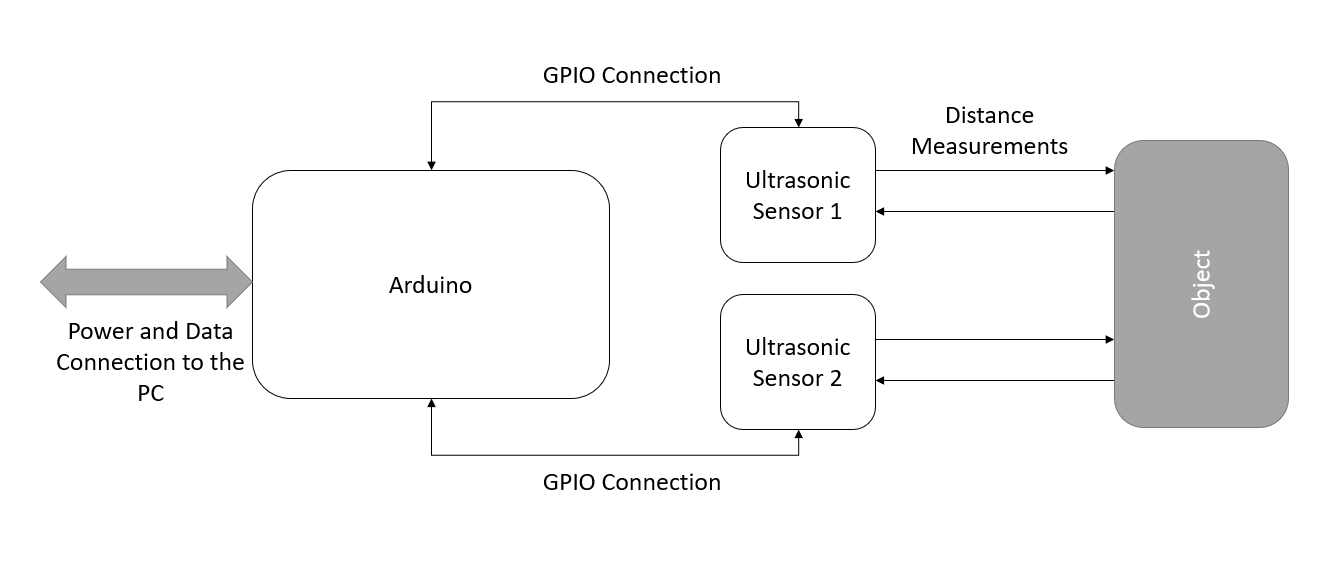
\includegraphics[width=8.5cm, height=6cm]{images/data_collection_block.png}
\centering
\caption{Block Diagram for a Constrained Device}
\label{fig:collection1}
\end{figure}

Data were collected for a number of obstacles, namely a closed door, a display stand, a storage box, and a large bin, with each obstacle placed in the centre of a hallway. These obstacles were chosen because they are reasonably large, and as such, should return strong distance measurements. 

In front of the obstacle was an imaged 3-foot by 3-foot grid. This grid was broken into 1-foot by 1-foot grids. This gives 9 grids in total, labelled 1 to 9. The data collection system will be placed in each of those 9 grids, pointing directly forward. When the measurement starts, it will be sent to a serial port monitor, specifically Tera Term. Tera Term allows the user to set up a file in which the transmitted data will be saved in comma-separate values (CSV) files. As well as the obstacles, data will be collected from the hallway when there is no object in place. As well as the gathered distance measurements information was gathered on the grid location and if an object was present or not. This information was output via a program written for the Arduino. An example of the dataset headers can be seen in Table \ref{table:1}:

\begin{table}[ht]
\centering
\begin{tabular}{||c c c c||} 
 \hline
 Channel1 & Channel2 & Object & Grid \\ [0.5ex] 
 \hline\hline
 2243 & 1392 & Yes & 1 \\ 
 \hline
 2399 & 1476 & Yes & 1 \\
 \hline
 2313 & 1245 & Yes & 1 \\
 \hline
 2257 & 1388 & Yes & 1 \\ [1ex] 
 \hline
\end{tabular}
\caption{Example of Ultrasonic Dataset}
\label{table:1}
\end{table}

\subsection{Initial Analysis}
\subsubsection{Introduction}
This section of the report will give a brief overview of the initial data analysis steps taken and the results generated from this analysis. This analysis will be carried out with a focus on what is referred to as "object analysis" and "grid analysis". The purpose of object analysis is to understand how well the machine learning techniques are at determining if an object is present or not in the data. Grid analysis is trying to determine how well machine learning or deep learning techniques can be used to determine how accurate the model is at determining which grid the data was gathered from. This information would be useful for navigation (i.e. should the person move to the left or right to avoid an object).

\subsubsection{Binary Analysis}
To understand how well a system may be able to detect an object or not, an initial test was carried out on the datasets. This initial examination would be carried out by using two datasets at a time: one dataset would be a dataset for an object, and the other dataset would be data gathered for no object. 

The data was processed through a number of classification models, specifically:
\begin{itemize}
    \item Logistic Regression
    \item Decision Tree
    \item K-nearest neighbour
    \item Linear discriminant analysis
    \item Gaussian Naive Bayes
\end{itemize}

The order of the datasets tested is shown in Table \ref{table:2}:
\begin{table}[ht]
\centering
\begin{tabular}{||c c||} 
 \hline
 Dataset 1 & Dataset 2  \\ [0.5ex] 
 \hline\hline
 Display Stand & Clear Hallway  \\ 
 \hline
 Closed Door & Clear Hallway \\
 \hline
 Storage Box & Clear Hallway \\
 \hline
 Large Bin & Clear Hallway \\ [1ex] 
 \hline
\end{tabular}
\caption{Datasets test for initial analysis}
\label{table:2}
\end{table}

The data was split using \texttt{train\_test\_split} with a 25 per cent split.

The results of this analysis can be seen in Fig. \ref{fig:init_binary}
\begin{figure}[h]
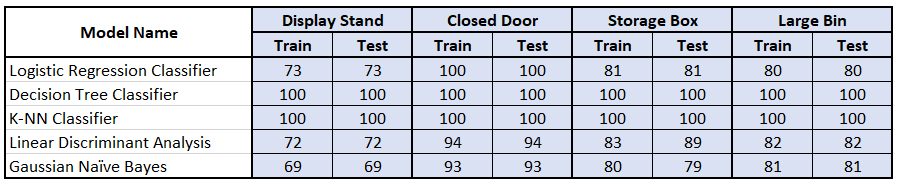
\includegraphics[width=8cm, height=3cm]{images/initial_binary_search.png}
\centering
\caption{Results for the Initial Binary Search}
\label{fig:init_binary}
\end{figure}

It can be seen from the results in Fig \ref{fig:init_binary} that the \texttt{Decision Tree Classifier} and \texttt{K-NN Classifier} are producing the best accuracy scores, with 100\% accuracy, for all the test data. The lowest accuracy score was generated by the \texttt{LDA} algorithm, producing an accuracy score of 72\%. It can be seen that typically the accuracy generated for the train data and that generated for the data are the exact same. One reason for this could be that the data does not have enough variation to generate a test dataset that is sufficiently different. However, these results did provide confidence that a system could be designed to detect objects. 


% \section*{Acknowledgment}


%\section*{References}
\printbibliography
\vspace{12pt}

\end{document}